\chapter{Beam Propagation}
\section{Gaussian beam}
Gaussian beam is an ideal beam used in optics to simplify calculations.

If we assume a Gaussian beam and no aperture, figure \ref{fig:gbna}.
\begin{figure}[h!]
    \centering
    \includegraphics[width=0.6\textwidth]{slike/gbna.pdf}
    \caption{Gaussian beam with no aperture}
    \label{fig:gbna}
\end{figure}

Electric field at aperture is $E(x) = \sqrt{I_0} e^{-\frac{x^2}{w_0^2}}$, inserting it 
into equation \ref{eq:gbe1} and solving for every possible $x'$ and $d$ gives us a \textbf{Gaussian beam}.
% lectures only say gives us .... next slide -> Gaussain beam

\begin{equation}
    E_{\sum}
    \label{eq:gbe1}(x',d) = \int_{-\infty}^{+\infty} \frac{E(x)}{1+ \sqrt{ (x'-x)^2 + d^2}} e^{|\vec{k}|\cdot \sqrt{(x'-x)^2 + d^2}-\omega t } dx
\end{equation}

Figure \ref{fig:gaussbeam} shows the parameters of the Gauss beam, symbols are explained in table \ref{tab:gaussbeam}.
\begin{figure}[h!]
    \centering
    \includegraphics[width=0.9\textwidth]{slike/gaus_beam.pdf}
    \caption{Gauss beam and parameters}
    \label{fig:gaussbeam}
\end{figure}

\begin{table}[h!]
    \centering
    \begin{tabular}{|c|c|c|}
        \hline
        Parameter& Definition & Formula \\
        \hline
        $w(z)$ & Beam radius at $z$ & $w(z) = w_0 \sqrt{1 + \frac{z^2}{z_R^2}}$\\
        $\theta$ & Divergence angle & $\Theta = \frac{\lambda}{\pi w_0}$ \\
        $w_0$ & Beam waist & $w_0 = \sqrt{\frac{z_R \lambda}{\pi}}$\\
        $z_0$, $z_R$ & Rayleigh length & $z_R = \frac{\pi w_0^2}{\lambda}$ \\
        $\sqrt{2}w_0$ & Beam waist @ $z_R$ & $\sqrt{2}w_0$ \\
        R(z) & Wavefront curvature & $R(z) = z [ 1 + (\frac{z_R}{z})^2]$ \\

        \hline
    \end{tabular}
    \caption{Gauss beam parameters}
    \label{tab:gaussbeam}

\end{table}
\subsection{Parameters}

\subsubsection{Rayleigh length and beam waist}
\textbf{Beam waist} $w_0$ is the smallest radius of the beam - "focal spot". Laser intensity in this spot 
is the highest. Equation \ref{eq:inte} shows the strength of electric field at distance $x$.

\begin{equation}
    E(x,z) = \sqrt{I_0} e^{-\frac{x^2}{w_0^2}}
    \label{eq:inte}
\end{equation}
%z je argument funk. ni pa uporabljen?


\textbf{Rayleigh length} $z_R$ is the distance from the beam waist at which the intensity is halved.
It is calculated by equation \ref{eq:zR}.
\begin{equation}
    z_R = \frac{\pi w_0^2}{\lambda}
    \label{eq:zR}
\end{equation}

Rayleigh length is important for processing of rough surfaces because the beam diameter stays relatively  \textbf{constant and small}.

Beam radius depends on Rayleigh length and waist $w_0$, diameter $w(z)$ is calculated by \ref{eq:w}.
\begin{equation}
    w(z) = w_0 \sqrt{1 + \frac{z^2}{z_R^2}}
    \label{eq:w}
\end{equation} 
Beam power is equal to the integral of intensity over area given by $w$ - equation \ref{eq:beampower}.
\begin{equation}
    P_L(z) = \int_{0}^{\infty} I(r,z) \cdot 2 \pi r dr = 2\pi I_0(z) \int_{0}^{\infty}r e^{-\frac{2r^2}{w(z)^2}} dr = \frac{\pi}{2} w(z)^2 I_0(z)
    \label{eq:beampower} 
\end{equation}
If we assume energy conservation for any distance - equation \ref{eq:bp2}.
\begin{equation}
    P_L(z) = \frac{\pi}{2} w(z)^2 I_0(z) = \frac{\pi}{2} w(z)^2 I_0(z=0) \rightarrow I_0(z)=\frac{w_0^2}{w(z)^2} I_0(z=0)
    \label{eq:bp2}
\end{equation}
Power is \textbf{constant}, intensity changes. 

\subsubsection{ Divergence angle}
In the far field, where $z >> z_R$, we can simplify equation \ref{eq:w} to equation \ref{eq:ffw}.
\begin{equation}
    w(z >> z_R) =w_0 \sqrt{1 + \frac{z^2}{z_R^2}} \approx w_0 \frac{z}{z_R}
    \label{eq:ffw}
\end{equation}
Beam radius increases linearly, when $z >> z_R$, divergence in the far field is \ref{eq:ffd}.
\begin{equation}
    \theta = \underset{z >> z_R}{lim} \frac{w(z)}{z} = \frac{w_0}{z_R} = \frac{\lambda}{\pi w_0}
    \label{eq:ffd}
\end{equation}

Beam parameter product is:  $\theta w_0 = \frac{\lambda}{\pi} = const$

\textit{Note: The smaller the beam waist diameter the bigger the divergence (and vice versa).}


\section{Beam size}
Beam can be measured at any point of its height. In experiments the most convenient measurments 
height is at \textbf{half maximum}, this is called \textbf{Full Width Half Maximum}.
For mathematical operations, height of $\frac{1}{e^2}$ is used, which is 13.5\% of the peak.
Figure \ref{fig:beamFWHM} shows FWHM.
\begin{figure}[h!]
    \centering
    \includegraphics[width=0.5\textwidth]{slike/fwhm.pdf}
    \caption{FWHM}
    \label{fig:beamFWHM}
\end{figure}

For a rotationally symmetric Gaussian beam - $TEM_{00}$, there is a linear relationship 
between FWHM and beam radius - $FWHM = \sqrt{2 ln(2)}w(z) = 1.177 w(z)$.

\subsection{Higher order TEM}

Figure \ref{fig:hobtem} shows the Gaussian beam for higher order TEM. 
Symmetric beam can be radial or cartesian. 
Cartesian symmetry:
\begin{gather}
    w_{m,n} = w_{00} \sqrt{2s + 1}\\
    \Theta_{m,n} = \Theta_{00} \sqrt{2s + 1}
\end{gather} where $s = m,n$. For a cartesian system each direction is evaluated on its own.

% is m = n = s?
For radial symmetry:
\begin{gather}
    w_{p,l} = w_{00} \sqrt{2p + l + 1} \\
    \Theta_{p,l} = \Theta_{00} \sqrt{2p + l + 1}
\end{gather}

\begin{figure}[h!]
    \centering
    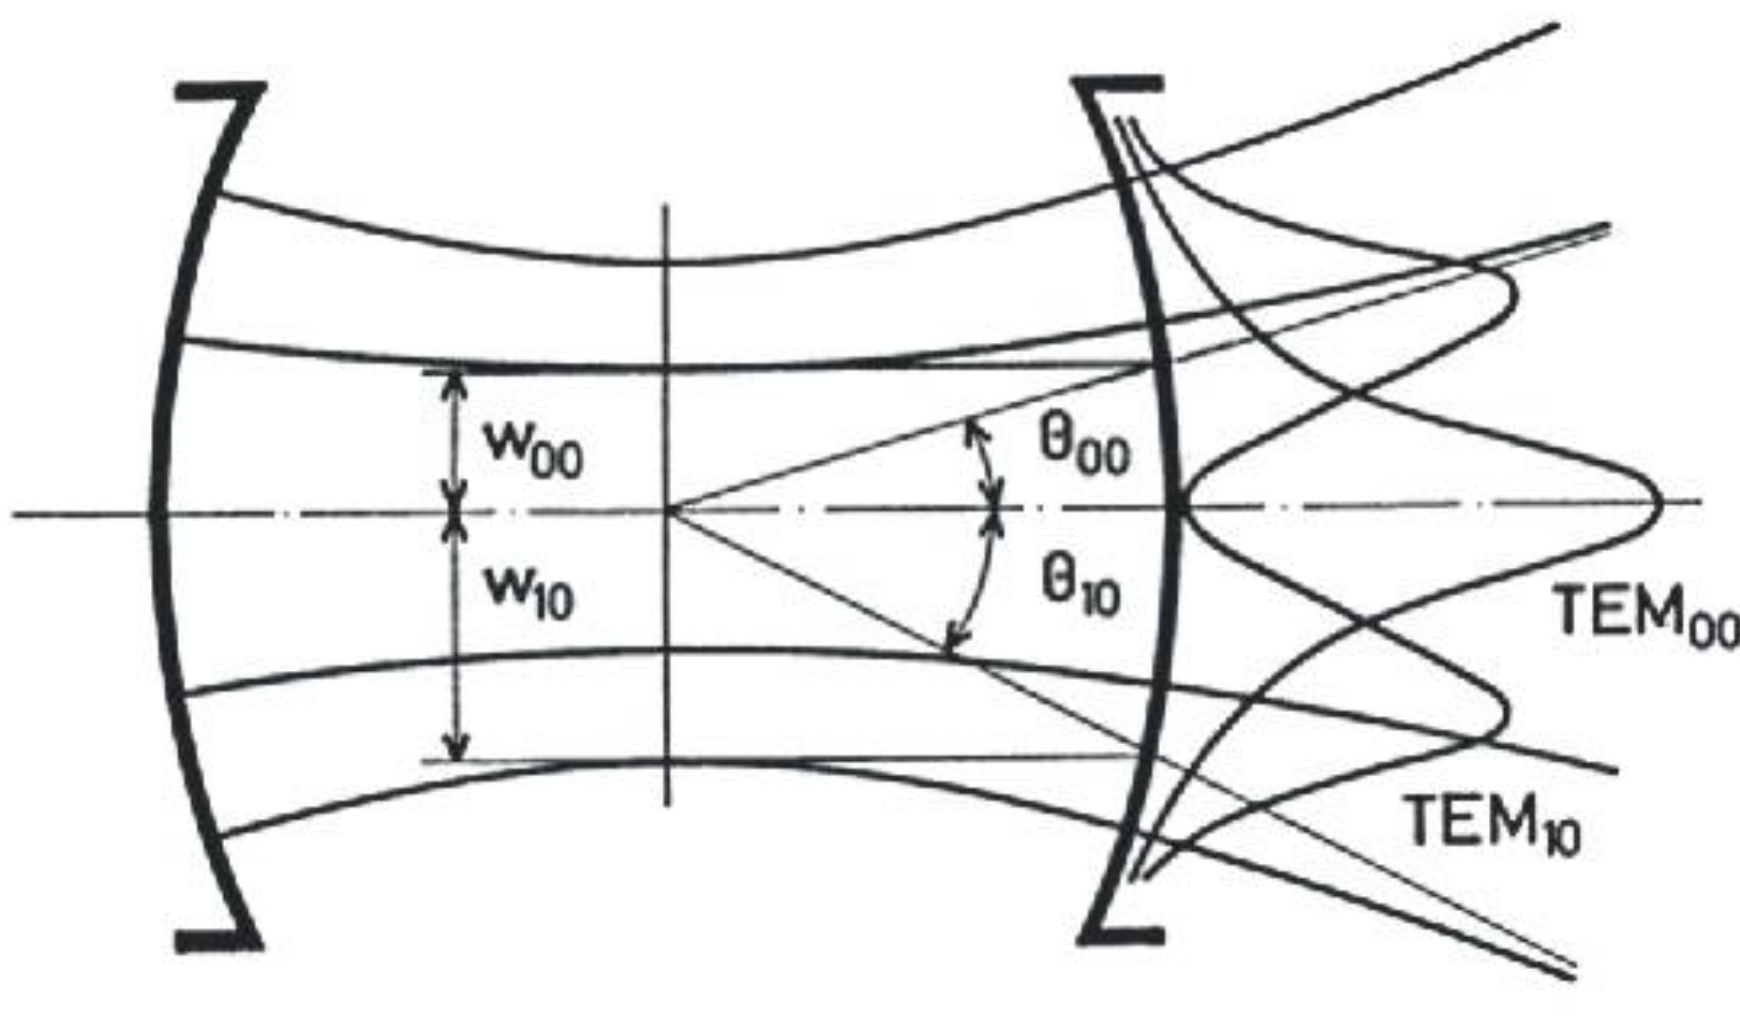
\includegraphics[width=0.5\textwidth]{slike/hobtem.png}
    \caption{Higher order TEM Gauss beam. \textit{Source: Lecture notes} }
    \label{fig:hobtem}
\end{figure}
 
Beam radius and divergence angle increases by a factor given by the mode structure.\\
\textbf{Conclusions}:
\begin{itemize}
    \item Focal spots for higher order modes are larger than for $TEM_{00}$ mode
    \item Higher order modes diverge faster than $TEM_{00}$ mode
    \item Higher order modes diverge differently
\end{itemize}

\section{Beam quality}
Beam propagation is simplified with a \textbf{beam quality factor} $M^2$.
Equation \ref{eq:M2} shows the definition.
\begin{equation}
    M^2 = \frac{(\Theta w)_{real}}{(\Theta_0 w_0)_{Gauss}}
    \label{eq:M2}
\end{equation}

For a Gauss beam whose  $M^2 = 1$ beam parameter product (BPP) is the smallest possible. 
All real beams have $1 < M^2 $. Ideal optical elements do not change the beam quality factor. 

Higher bam quality means:
\begin{itemize}
    \item Smaller focus diameter $\rightarrow$ higher intensity, lower divergence, better quality \dots
    \item Longer working distance $\rightarrow$ increased process stability, reduced risk for damaging optical components \dots
    \item Smaller optics $\rightarrow$ cheaper, more efficient cooling \dots
\end{itemize}

\textit{Note: in calculations $M^2$ is always multiplied with $\lambda$}.

\section{Focusing of Gaussian beams}

Due to optical aberrations/imperfections and diffraction, limited spot sizes are 
not achievable. Both increase the $M^2$ and the beam parameter product.
Equation \ref{eq:rbeam} shows the waist size accounting for imperfections.

\begin{equation}
    w_f = \textcolor{black}{\frac{2\lambda}{\pi} \cdot \frac{f}{D} \cdot M^2} + \textcolor{blue}{ C_L \cdot \frac{D^3}{f^2} }
    \label{eq:rbeam}
\end{equation}
Where $D$ is the laser beam diameter.  Figure \ref{fig:saber} show the spherical aberration, which also increases $M^2$, coloured blue in equation \ref{eq:rbeam}.


\begin{figure}[h!]
    \centering
    \includegraphics[width=0.3\textwidth]{slike/saberation.pdf}
    \caption{Spherical aberration}
    \label{fig:saber}
\end{figure}

If the following beam properties:
\begin{itemize}
    \item Short wavelength
    \item Short focal length
    \item Large beam diameter
    \item Using well suited lens combinations
\end{itemize}
Are present, we can simplify the equation \ref{eq:rbeam} to $w_f = \textcolor{black}{\frac{2\lambda}{\pi} \cdot \frac{f}{D} \cdot 1}$, as the other parameters are negligible.

\section{Gaussian beam propagation}

Figure \ref{fig:gbp} shows the effect a lens has on a  plane wave beam.
\begin{figure}[h!]
    \centering
    \includegraphics[width=0.5\textwidth]{slike/gaussbeampropagation.pdf}
    \caption{Gauss beam propagation}
    \label{fig:gbp}
\end{figure}

Lens imposes a curvature on the beam, equation \ref{eq:Rlns}. Change in curvature imposed by the propagation in free space
is given by equation \ref{eq:Rfree}
\begin{equation}
    R_{new} = R_{old} + f
    \label{eq:Rlns}
\end{equation}
\begin{equation}
    R(z) = z (1 + \frac{z_R^2}{z^2})
    \label{eq:Rfree}
\end{equation}
Combining equations leads to equation \ref{eq:Rnew}.
\begin{equation}
    \frac{1}{R_{new}} = \frac{1}{z (1 + \frac{z_R^2}{z^2})} + \frac{1}{f_{@z}}
    \label{eq:Rnew}
\end{equation}

To separate curvature and beam size, we use \textit{complex numbers}.

\subsection{Complex q-parameters}
Complex parameter q is defined by equation \ref{eq:qparm}.
\begin{equation}
    \frac{1}{q(z)} = \frac{1}{(z + \frac{z_R^2}{z})} - i \frac{1}{z^2 + z_R^2} = \frac{1}{R(z)} - i \frac{\lambda}{\pi w(z)^2}
    \label{eq:qparm}
\end{equation}
Which is equal to \ref{eq:qinv}.
\begin{equation}
    q(z) = \frac{\frac{1}{R}}{R^2 + (\frac{\lambda}{\pi w^2})^2} + i \frac{\frac{\lambda}{\pi w^2}}{R^2 + (\frac{\lambda}{\pi w^2})^2}
    \label{eq:qinv}
\end{equation}

New free space propagation equation is $q(z) = z + i z_R$. \textbf{Real part} of $\frac{1}{q}$ is the \textbf{curvature}, \textbf{imaginary part} is the \textbf{site of beam} at z.

\subsubsection{Q-parameter at lens}
Real part of $\frac{1}{q}$ is equal to zero. Lens changes the curvature to the radius of $f$. New real 
part is therefore $\frac{1}{f}$. If the beam already has a curvature before the lens, 
the lens will make curvature even smaller, according to equation \ref{eq:qlens}.
\begin{equation}
    \frac{1}{q_{out}} = 0 + i \frac{1}{z_R} + \frac{1}{f} = \frac{1}{q_{in}} + \frac{1}{f}
    \label{eq:qlens}
\end{equation}

At position $z=0$ the curvature is infinite, q parameters are equal to:
\begin{equation}
    \frac{1}{q(z=0)} = 0 + i \frac{1}{z_R}
\end{equation}

We can also use \textit{q parameters} with the ABCD matrix computation, $q_f$ is equal to
\begin{gather}
    q_f = \frac{A q_i + B}{C q_i + D} \\
    \frac{1}{q_f} = \frac{C + D/q_i}{A + B/q_i}
\end{gather}
